\section{Benefits}
\begin{table}[htbp]
  \centering
  \caption{Overview of capacitive proximity sensing benefits}
    \begin{tabular}{p{4cm}p{6cm}}
    \toprule
    \textbf{Name} & \textbf{Examples} \\
    \midrule
    \textbf{Versatility} & Flexible electrode design, scalability, different sensing methods \\
    \textbf{Unobtrusiveness} & Invisible application, non-disturbing frequency range \\
    \textbf{Processing Complexity} & Small number of sensors, variable dynamic range \\
    \bottomrule
    \end{tabular}%
  \label{tab:cap_benefits}%
\end{table}%

Given the information collected in the previous section we can now talk about the specific benefits of capacitive proximity sensing. We are using three different groups for categorization, namely versatility, unobtrusiveness and processing complexity. Some examples within these groups are shown in Table \ref{tab:cap_benefits}. In the following section I will discuss those groups in detail.
\subsection{Versatility}
A main benefit of capacitive proximity sensors is the versatility in which they can be applied. With flexible choice of electrode materials, size and geometry it is possible to create highly individual applications. Example electrodes include transparent metal oxide layers, woven conductive thread, copper wires, PCB boards or simple aluminum foil. In the different prototypes we have used all varieties of materials, including aluminum foil in the MagicBox (\ref{ch:prot_magicbox}), long copper wire electrodes in the CapFloor (\ref{ch:prot_magicbox}), conductive thread in the Capacitive Chair (\ref{ch:prot_magicbox}) and transparent ITO in GestDisp (\ref{ch:prot_otherprot}). Other materials in the literature include plant tissue for Botanicus Interactus \cite{poupyrev2012botanicus} and water in Touché \cite{Sato2012}. The size and shape of the electrodes is varying accordingly. The finger tracking array in the Active Armrest (\ref{ch:prot_armrest}) consists of 2 cm x 3 cm copper PCB, while the Capacitive  Chair (\ref{ch:prot_capchair}) has some electrodes of 15 cm x 20 cm. The largest electrodes of the related works can be found in the TileTrack prototype using 60 cm x 60 cm tiles \cite{valtonen2010human}. The electrode design can be modified freely according to the specific application scenario. Given the large variety of different sensing methods most scenarios can be covered.

Additionally, the sensor systems are also highly scalable. By choosing appropriate voltages and frequencies it is possible to add a high number of sensors to a single object. Rekimoto's SmartSkin uses shunt mode, with nine emitters and eight receivers leading to 72 sensing points \cite{rekimoto2002smartskin}. The CapTap prototype uses three OpenCapSense boards, interfacing 24 sensors, relying on time multiplexing to prevent interference between the different sensors (\ref{ch:prot_captap}). The CapFloor prototype as used in the EvAAL competition connected 26 sensors to a single PC system, controlled by two different communication interfaces (\ref{ch:prot_capfloor}). Further iterations developed by Tobias Grosse-Puppendahl support 100+ sensors in setups covering multiple rooms. Using smart measurement windows and different multiplexing methods, sensors can be placed close together and electrodes may act as both sender and receiver, e.g. the frequency multiplexing method used in the Honeyfish system \cite{grosse2012honey} (\ref{ch:prot_otherprot}). The different sensing methods presented - loading mode, shunt mode and transmit mode enable a variety of different sensing patterns. The human body can be used as both sender and receiver and smart electrode layouts allow using low-powered processors. 

In conclusion, it is possible to add capacitive sensing to most everyday objects to enable different forms of interaction, create natural interfaces and smart objects. Our prototypes are using different electrode materials, flexible or solid electrodes, conductive thread, wires, shielded or non-shielded layouts.
 
\subsection{Unobtrusiveness}
\begin{minipage}{\linewidth}
\centering
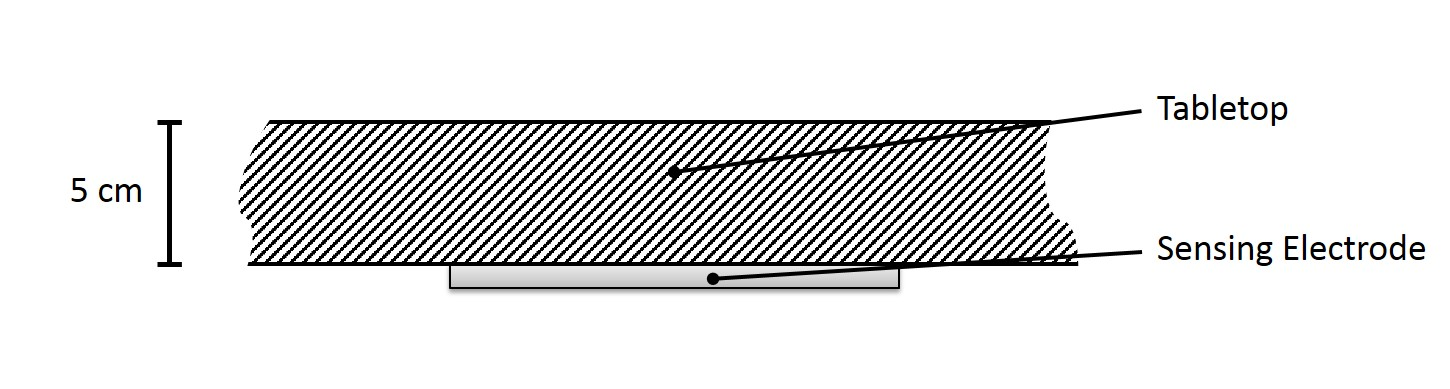
\includegraphics[width=0.8\textwidth]{images/eval_unobtrusive}
\captionof{figure}{Sketch of CapTap prototype showing thickness of tabletop}
\label{fig:eval_unobtrusive}
\end{minipage}

Electric fields are not usually perceived by persons, unless they are of exceptional strength. Capacitive proximity sensors usually operate with low voltages (OpenCapSense operates at 3.3 V or 5 V) and with frequencies that are not considered biologically active (OpenCapSense uses a 100 kHz sampling rate). Furthermore, they propagate through many materials that are typically present in our environment, including most plastics, wood or tile. This allows us to invisibly apply capacitive proximity sensors without a strong effect on the measurement. Regarding the Smart Bed (\ref{ch:prot_smartbed}) the signal propagates through a thick layer of mattress, consisting of polyurethane foam. The CapFloor system is designed to work below wood, PCV, tile, or other non-conductive floor materials (\ref{ch:prot_capfloor}). Application below several centimeters of covering is possible, if the electrodes are designed properly for large distance sensing. The detection range of the CapTap demonstrator is not disturbed by the laminated wood tabletop of 5 cm thickness (\ref{ch:prot_captap}). Similar the Capacitive Chair has electrodes attached below a cover comprised of wood, polyurethane foam and cloth, the materials of the seat area (\ref{ch:prot_capchair}). Other materials that were applied above capacitive proximity sensors in the scope of the experiments were glass, polycarbonate, carpet, or access floors, comprised of a wood, plastic and carpet combination. None of the materials we used showed unexpected behavior, related to absorption or attenuation of the sensor signal. If the sensors are attached close to conductive materials the signal can be disturbed if they are grounded or acting as shield towards the object to be sensed. Shielding in this context describes preventing the electric field created by the sensors to propagate to the object that is supposed to be detected, e.g. the famous Faraday cage. In some scenarios capacitive proximity sensors can also be used to detect properties of conductive objects, e.g. it is possible to detect the level of water in a glass or other non-conductive container.

It is possible to equip most conductive objects directly with capacitive proximity sensors and hide them below non-conductive objects with minimal spatial requirements. The Active Armrest (\ref{ch:prot_armrest}) prototypes are using sensor sets that are completely invisible from the outside.  The CapTap was specifically designed to combine several sensing technologies that are invisible from the outside - hidden electrodes and a microphone (\ref{ch:prot_captap}). The thickness of the tabletop is shown in Figure \ref{fig:eval_unobtrusive}. One disadvantage of this method is the disability to easily detect touch if there is no contact between object and electrode. Touching the electrode will typically cause a spike in sensor values that can be very easily discriminated. Therefore, in order to detect touches narrow thresholds and suitable sensing electrodes have to be used, as shown in SmartSkin \cite{rekimoto2002smartskin} or the touch area of the Active Armrest (\ref{ch:prot_armrest}). Another potential solution is to use indirect effects of touching. The Smart Bed is using the pressure applied on the mattress to cause a geometric deformation of the electrode (\ref{ch:prot_smartbed}). This results in a clearly measurable spike in sensor values and can be modified for application below other flexible surfaces.
The Smart Bed is additionally designed to communicate wireless to a PC only using a regular power supply for operation.
 
\subsection{Processing Complexity}
An appropriate analogy to capacitive proximity sensors is a single photo diode. As opposed to a light intensity, capacitance is measured. While the information we can gain from such a measurement is limited, the processing required to analyze the signal is also low. Performing signal analysis on an array of 24 capacitive sensors, as in the CapTap prototype (\ref{ch:prot_captap}) is comparable to processing the image of a 6x4 pixel camera. Therefore, it is easy to create highly integrated systems with low-power devices for performing any subsequent data analysis. Other prototypes use even less electrodes, most notably the Magic Box that uses only six sensors and computationally inexpensive object localization algorithms (\ref{ch:prot_magicbox}. 

While it is possible and in many cases beneficial to use complex data processing algorithms for object detection, it is in many cases possible to achieve a similar result with less complex methods. In many applications it is even viable to opt for a quantized capacitance measurement. In the case of a touch sensor a single binary measure is sufficient. However, it is also possible to select various different levels. The Active Armrest processes the two back electrodes in a quantized fashion, just using a single threshold for each (\ref{ch:prot_armrest}). The sensor dynamic can be reduced to any suitable range, thus reducing the processing complexity later in the algorithms. The CapFloor system uses a larger number of sensors and does not require a high dynamic range for calculations  (\ref{ch:prot_capfloor}) and thus uses shortened 4 Bit values.

With the exception of the Capacitive Chair (\ref{ch:prot_capchair}) and the CapTap (\ref{ch:prot_captap}) that make extensive use of frequency domain operations, our prototypes are using simple data processing methods that can be easily applied on embedded systems. One of the presented examples is the weighted average algorithm for object detection, as shown for the Magic Box (\ref{ch:prot_magicbox}). Regarding model-based data processing, even very simple cylindrical models, such as the one used for the Smart Bed (\ref{ch:prot_smartbed}), are capable to reliably predict numerous postures that are relevant in real world applications. In general, the low requirements for data pre-processing, allows dedicating more resources to high-level data processing algorithms if the specific application is resource constrained. Thus, it is easily possibly to fuse the data of multiple heterogeneous sensors in the system or apply more complex classification methods, such as the SVM classifier used for the Capacitive Chair (\ref{ch:prot_capchair}).

Another option to reduce the processing load is reducing the sample rate of the sensors. If this is done in hardware there is an additional benefit to this method. The sensitivity of the sensors can be increased, as loading and unloading times can be decreased, making it easier to detect changes in the resulting capacitance. However, this method is not used for all potential electrode sizes, as particularly small electrodes will reach their capacitance limit fairly early. Another option to increase the sensitivity is increasing the voltage that influences the propagation range of the electric field. In this case it is more difficult to guarantee biological inactivity and a low power consumption.

The OpenCapSense toolkit that is the base for most of the prototypes has a fairly powerful micro controller that is able to implement all of the processing steps - thus enabling highly integrated, low-power capacitive proximity sensing prototypes that can be used in smart environment applications. It is viable to use very low-powered PC systems, such as the Raspberry Pi to interface a large number of capacitive proximity sensors in research applications.
